\section{Assembly and Execution}
\label{sec:Durchfuehrung}
\subsection{Assembly}
The diode laser and all other instruments are set up on an optical table.
To discern where the diode laser is pointing a special card was given to us which turns the non-visible light from the laser into visible light.
Further a CCD-camera connected to a screen is used to broadcast a live video of the light spot on the card or the fluorescence in the cell to get a more convenient look at them.
The rubidium gas is confined to a cell whose temperature is regulated via a control panel.
The diode laser itself can be rotated in the horizontal plan via a side knob.
This causes a variation of length for the external cavity as well as the angle between the diode and the grating which in turn causes a change in frequency of the laser.

\subsection{Determination of the Threshold Current}
\label{sec:threshold}
At first the threshold current $I_{\text{th}}$ at which lasing takes place has to be determined.
As seen in \autoref{fig:assembly1} a card is placed so that it intercepts the laser beam and the camera is focused on the card.
Now the current is steadily increased from zero.
In the beginning a light spot is visible on the card.
This means that the diode laser only acts as an LED.
But when a certain threshold current is passed the light spot suddenly gets brighter and a speckle pattern can be observed.
\begin{figure}
    \center
    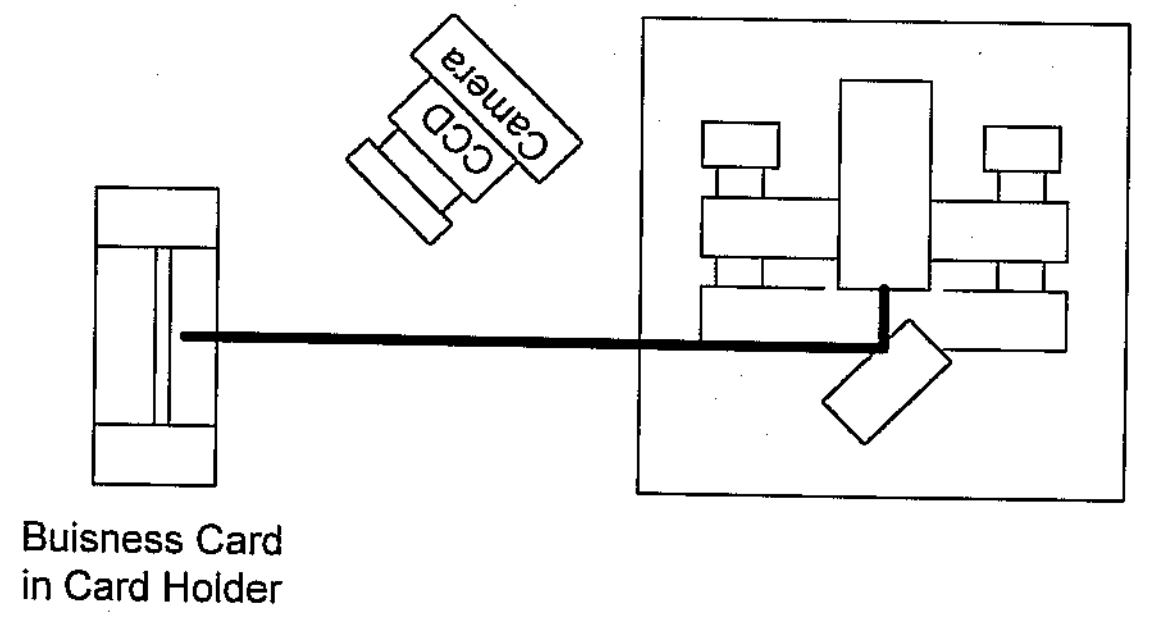
\includegraphics[width=0.8\textwidth]{bilder/Assembly_1.png}
    \caption{Assembly containing the diode laser, the camera and the card to determine the threshold current. \cite{anleitung}}
    \label{fig:assembly1}
\end{figure}

\FloatBarrier

\subsection{Rubidium fluorescence}
Next, you set up a rubidium cell so that the laser beam passes through it like in \autoref{fig:assembly2}.
The camera is now aligned vertically to the direction of propagation as it is focused on the cell.
The current is set significantly higher than the threshold current.
The side knob is now used to adjust the horizontal position and thus the frequency of the external cavity.
A piezoelectric stack scans a comparably small part of the frequency spectrum by moving the optical feedback grating with a certain frequency.
By changing these two parameters, the horizontal position and the frequency of the piezo, it is achieved that the rubidium fluorescence is seen at all times.
\begin{figure}
    \center
    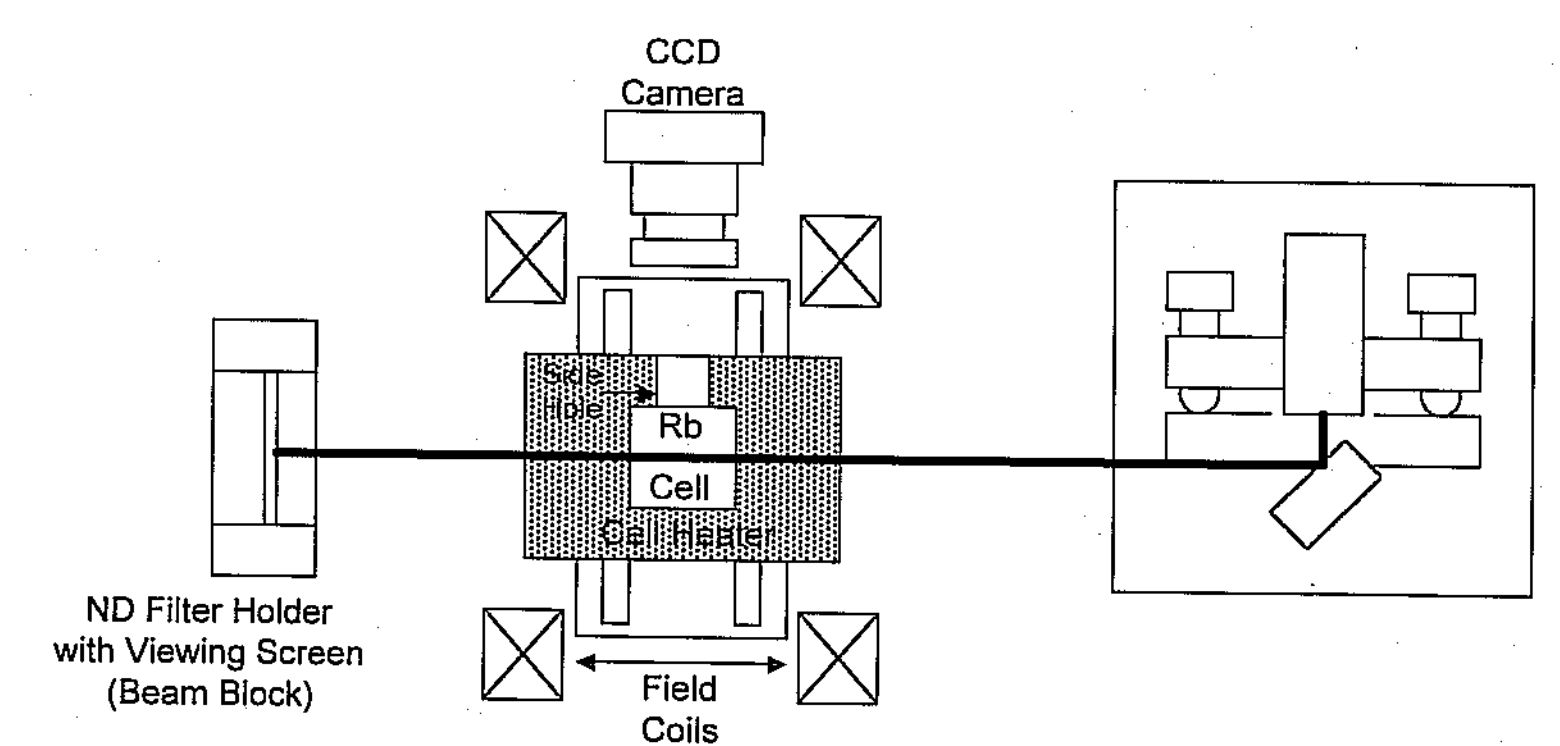
\includegraphics[width=0.8\textwidth]{bilder/Assembly_2.png}
    \caption{Assembly containing the diode laser, the camera, the card and the rubidium cell to observe rubidium fluorescence. \cite{anleitung}}
    \label{fig:assembly2}
\end{figure}

\FloatBarrier

\subsection{Absorption spectrum of Rubidium}
\label{sec:absorption}
As seen in \autoref{fig:assembly3} the beam passing through the cell is intercepted by a photodiode which turns the intensity of the laser beam to a proportional voltage.
This voltage is displayed on the screen of a connected oscilloscope.
Since the photodiode is very sensible to ambient light the room is darkened.
On the oscilloscope can now be seen various peaks and mode hops.
The second photodiode is aimed at with a 50/50-beam-splitter positioned in between the diode laser and the rubidium cell which lets through half of the laser light and reflect the other half.
To eliminate external influences the signals of both photodiodes are subtracted from one another.
Lastly the absorption spectrum on the oscilloscope is chosen by varying the current, the piezo and the side knob (and the oscilloscope settings) so that no mode hops and all four, maximally visible absorption peaks can be observed.
\begin{figure}
    \center
    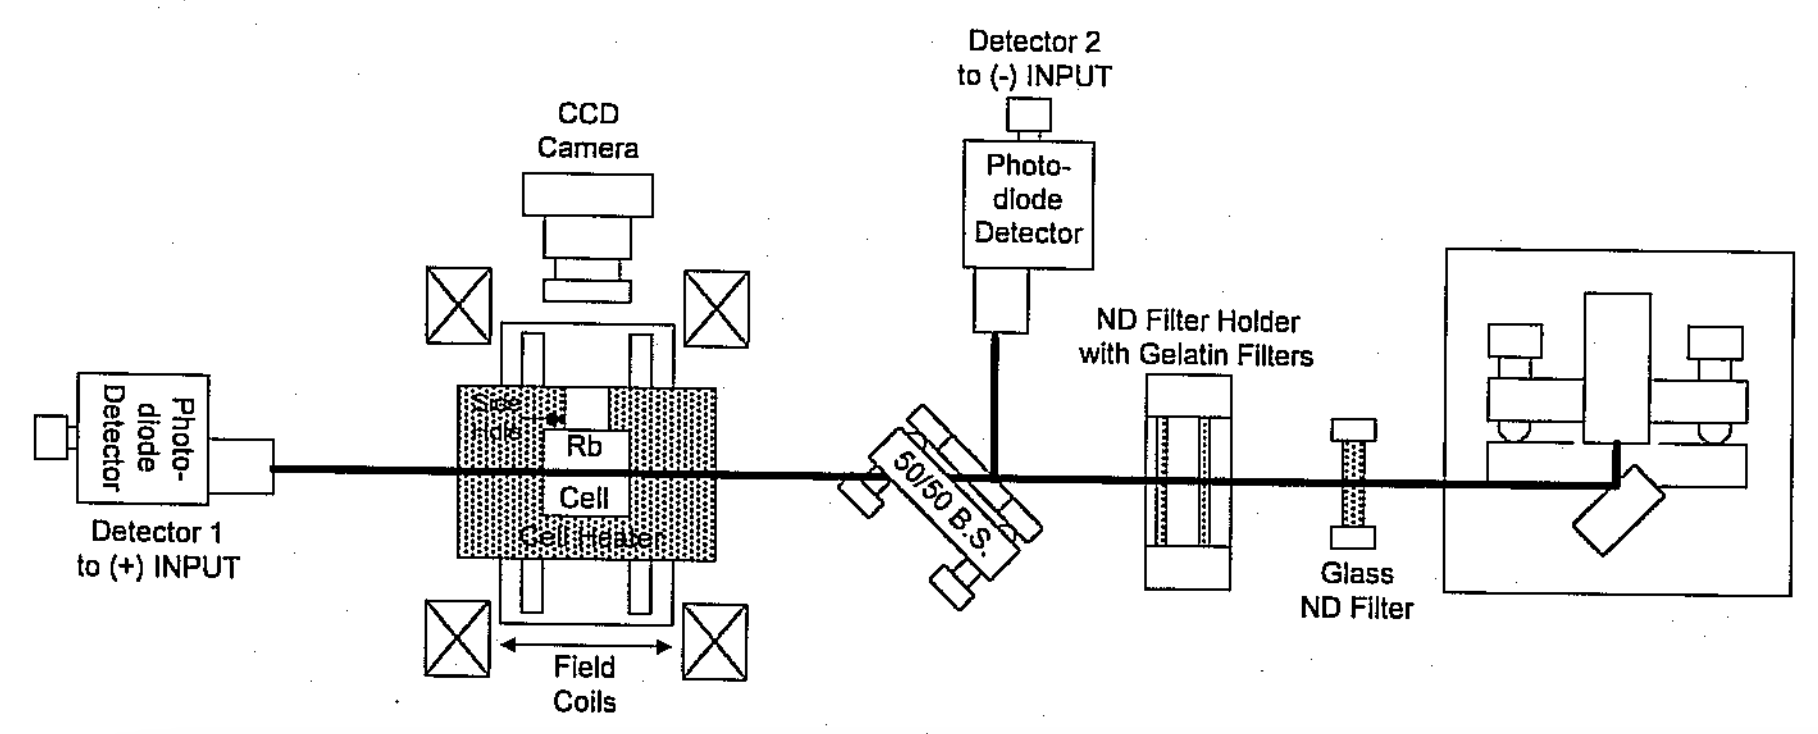
\includegraphics[width=0.8\textwidth]{bilder/Assembly_3.png}
    \caption{Assembly containing the diode laser, two photodiodes, the 50/50-beam-splitter and the oscilloscope to get the absorption spectrum of rubidium. \cite{anleitung}}
    \label{fig:assembly3}
\end{figure}

\FloatBarrier
